
%(BEGIN_QUESTION)
% Copyright 2010, Tony R. Kuphaldt, released under the Creative Commons Attribution License (v 1.0)
% This means you may do almost anything with this work of mine, so long as you give me proper credit

Suppose the feedback bellows in this pneumatic controller were replaced with one significantly smaller (having a much smaller surface area for air pressure to act upon, and also a much smaller internal volume):

$$\includegraphics[width=15.5cm]{i01768x01.eps}$$

Identify the effects this component change would have on the controller, and on the process being controlled:

\vskip 10pt

\begin{itemize}
\item{} Will this alteration {\it increase}, {\it decrease}, or {\it not affect} the proportional band of the controller?
\vskip 10pt
\item{} Will this alteration {\it increase}, {\it decrease}, or {\it not affect} the bias value in the controller's equation?
\vskip 10pt
\item{} Will this alteration {\it increase}, {\it decrease}, or {\it not affect} the time it takes for the controller's output to fully respond to a sudden change in PV or SP signal?
\vskip 10pt
\item{} Assuming the controller did a fine job controlling the process before this component change, describe how this alteration will affect the quality of control:
\end{itemize}

\underbar{file i01768}
%(END_QUESTION)





%(BEGIN_ANSWER)

\begin{itemize}
\item{} This alteration will {\bf decrease} the proportional band of the controller.
\vskip 10pt
\item{} This alteration will {\bf increase} the bias value in the controller's equation.
\vskip 10pt
\item{} This alteration will {\bf decrease} the response time of the controller to a sudden change in PV or SP signal.
\vskip 10pt
\item{} Assuming the controller did a fine job controlling the process before this component change, this alteration will cause the control quality to be over-reactive (oscillatory) and also develop less PV $-$ SP offset than before.
\end{itemize}

%(END_ANSWER)





%(BEGIN_NOTES)


%INDEX% Control, proportional: pneumatic force-balance controller

%(END_NOTES)


